\documentclass{report}
\usepackage[margin=1in, paperwidth=8.5in, paperheight=11in]{geometry}
%Math packages%
\usepackage{amsmath}
\usepackage{amsthm}
%Spacing%
\usepackage{setspace}
%Package to adjust indentation%
\usepackage{changepage}
\onehalfspacing
%Lecture number%
\newcommand{\lectureNum}{20}
%Variables - Date and Course%
\newcommand{\curDate}{March 21, 2017}
\newcommand{\course}{CS 240}
%Defining the example tag%
%\theoremstyle{definition}%
\newtheorem{ex}{Example}[section]
%Setting counter given the lecture number%
\setcounter{chapter}{\lectureNum{}}
%Package to insert code%
\usepackage{listings}
\usepackage{courier}
\usepackage{xcolor}
\lstset { 
    tabsize=2,
    breaklines=true,
    language=C++,
    backgroundcolor=\color{blue!8}, % set backgroundcolor
    basicstyle=\footnotesize\ttfamily,% basic font setting
}
%Package to draw trees%
\usepackage{tikz}


\begin{document}
%Note title%
\begin{center}
\begin{Large}
\textsc{\course{} | Lecture \lectureNum{}}
\end{Large}
\end{center} 
\noindent \textit{Bartosz Antczak} \hfill
\textit{Instructor: Eric Schost} \hfill
\textit{\curDate{}}
\rule{\textwidth}{0.4pt}
% Actual Notes%
\section{Compression}
This section focuses on how we store and transmit data. We'll focus mainly on encoding and decoding text by using algorithms. Other than measuring the efficiency of these algorithms, we can also measure:
\begin{itemize}
\item Processing speed
\item Reliability
\item Security (i.e., how safe is the encryption, or encoded text)
\item Size
\end{itemize}
We define the compression ratio as:
$$\frac{|C| \cdot \log |\Sigma_C|}{|S| \cdot \log |\Sigma_S|}$$
($S$ represents the source text (i.e., text from the source alphabet $\Sigma_S$ that is about to be encoded; $C$ represents the encoded text from the coded alphabet $\Sigma_C$)
\subsection{Types of Data Compression}
\subsubsection{Logical vs. Physical}
\begin{itemize}
\item \textbf{Logical Compression:} uses the meaning of the data and only applies to a certain domain (e.g., sound recordings)
\item \textbf{Physical Compression:} only knows the physical bits in the data, not the meaning behind them
\end{itemize}
\subsubsection{Lossy vs. Lossless}
\begin{itemize}
\item \textbf{Lossy Compression:} achieves better compression ratios, but the decoding is approximate; the exact source text S is not recoverable
\item \textbf{Lossless Compression:} always decodes S exactly
\end{itemize}
We will concentrate on physical, lossless compression algorithms.\\
We will use ASCII to encode characters.
\subsection{Decoding}
To decode encoded text, we will use a decoding algorithm mapping $\Sigma_C* \rightarrow \Sigma_S*$ (the Kleene start represents every possible character in the respective alphabet).\\
Our code must be uniquely decodable, and it's helpful if a code is \textit{prefix-free}, which means that for any character in our encoded alphabet, there exists one and only one character in the decoded alphabet to map to ($\Sigma_C* \rightarrow \Sigma_S$). To understand why we need this, consider the following non-uniquely decodable mapping:
\begin{align*}
A &\rightarrow 1 \\
B &\rightarrow 0 \\
C &\rightarrow 01
\end{align*}
What if we wanted to encode the text 01? Do we map it to $C$ or $BA$? 01 is on trial right now, and (voice of Roger Waters) \textit{this will not do}.
\subsection{Huffman Coding}
Involves building a binary trie to store the decoding dictionary D. Each character of $\Sigma$ is a leaf of the trie.
\textbf{Encoding} a text simply involves finding the encoded text representation of each character in $\Sigma_S$.\\
\textbf{Decoding} a text involves reading the encoded text and tracking the characters in the trie. Once we hit a character, print that character, and repeat.
\begin{ex}
Huffman Coding trie with decoded alphabet $\Sigma_S = \{$\texttt{A,N,O,E,T,\_}\}
\end{ex}
\begin{figure}[ht]
\begin{center}
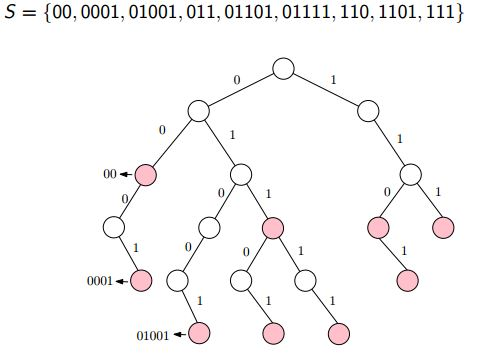
\includegraphics[scale=0.8]{trie1.jpg}
\end{center}
\end{figure}
\noindent Encoding \texttt{AN\_ANT} returns 01 001 000 01 001 11.\\
Decoding 11 100 000 101 01 11 returns \texttt{TO\_EAT}.
\subsection{Building the Best Trie}
For a source text S, how do we determine the best trie which minimizes the length of C?
\begin{itemize}
\item Determine the frequency of each character $c \in \Sigma_S$
\item Make $|\Sigma_S|$ trie of height 0 holding each character. Assign a weight to each trie, which is the sum of frequencies of all letters in the trie (initially, these are just the character frequencies)
\item Merge two tries with the least weights. Their new weight s their sum
\item Repeat the previous step until there is only one trie left
\end{itemize}

%END%
\end{document}